
\begin{wrapfigure}[17]{r}{0.55\textwidth}
		\vspace{-1.2cm}
        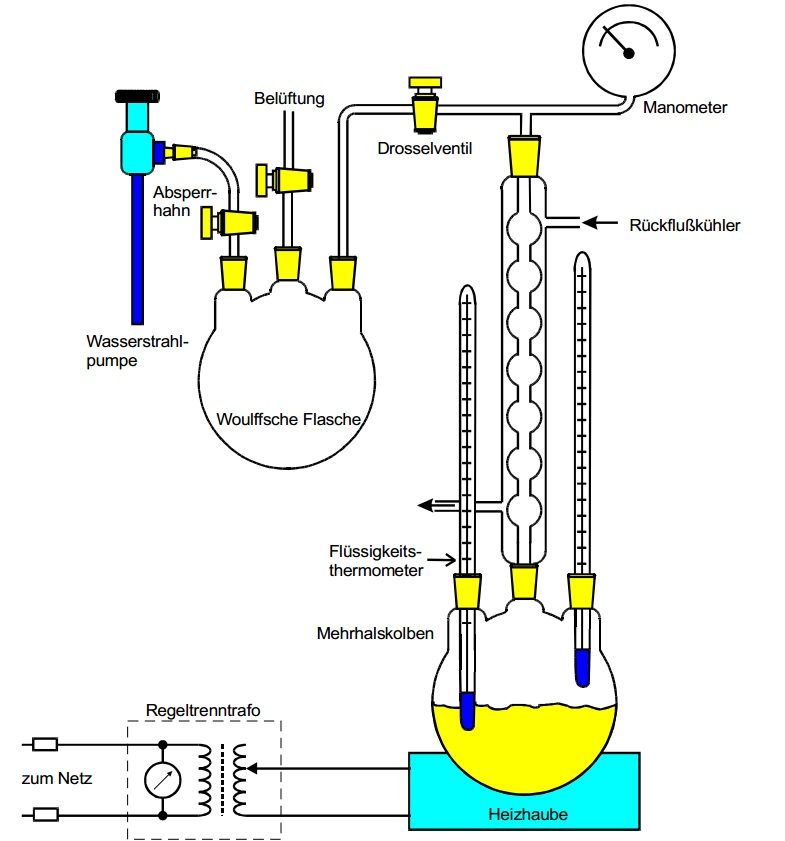
\includegraphics[width=0.55\textwidth]{Grafiken/Abb3.jpg}
        \caption{Schematische Darstellung der Messaparatur aus Versuchsteil 1 \cite{V203}}
        \label{fig:Abb3}
\end{wrapfigure}

Im ersten Versuchsteil (siehe \cref{fig:Abb3}) soll der Druck $p \leq \SI{1}{bar}$ sein.
Zunächst wird der Druck im Mehrhalskolben auf ca. $\SI{40}{mbar}$ verringert, 
dies geschieht durch Öffnen des Absperrhahns und Drosselventils und schließen des Belüftungsventils 
an der woulffschen Flasche, sobald dies durch die Unterzuhilfenahme der Wasserstahlpumpe geschehen ist, 
wird der Absperrhahn verschlossen und die Wasserstahlpumpe abgestellt, danach wird auch das Drosselventil geschlossen 
und der Mehrhalskolben erhitzt, dabei wird noch der Rückflusskühler eingestellt, bei ca. \SI{80}{\celsius} wird
der Rückflusskühler langsam gedrosselt, da sonst höhere Temperaturen nur schwer zu erreichen sind.
Die Temperaturen werden jetzt ca. alle 2 Grad an dem Thermometer im Gasraum und der Druck am Manometer abgelesen.\\

\begin{wrapfigure}[10]{r}{0.55\textwidth}
       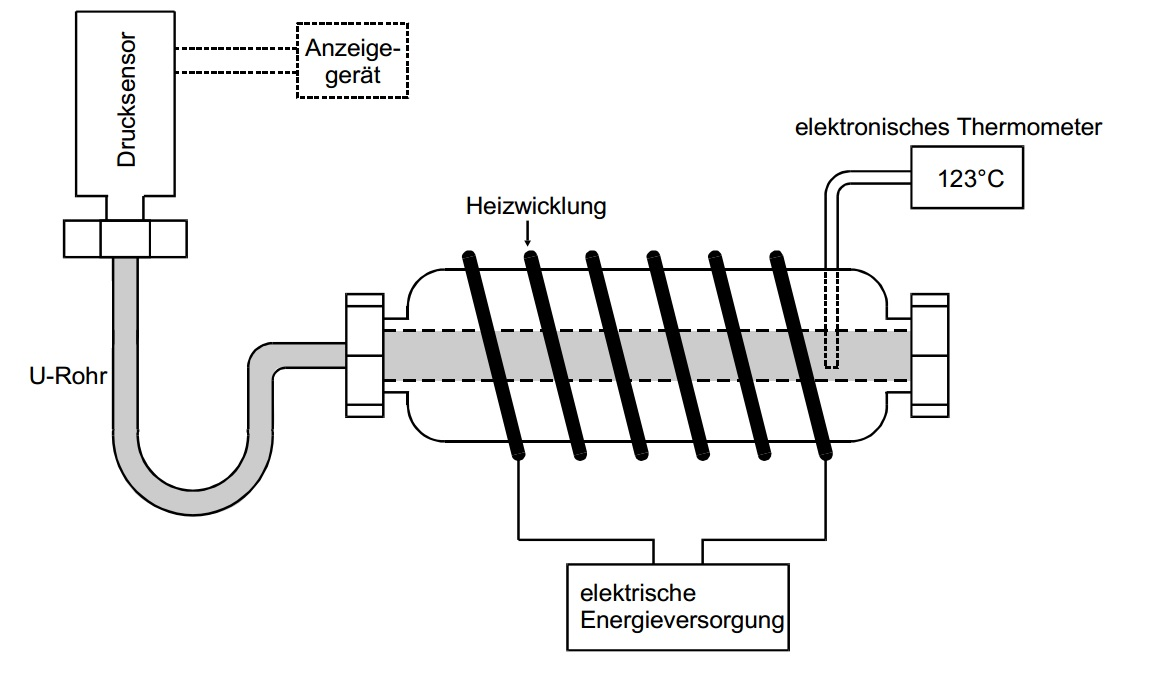
\includegraphics[scale=0.3]{Grafiken/Abb4.jpg}
        \caption{Schematische Darstellung der Messapparatur aus Versuchsteil 2 Schematische Darstellung der Messapparatur (leicht verändert)\cite{V203}}
        \label{fig:Abb4}
\end{wrapfigure}

Im zweiten Versuchsteil (siehe \cref{fig:Abb4}) wird der über den Aufbau für 
$p > \SI{1}{bar}$ bestimmt.
Bei dieser Messapparatur wird, entgegen der Anleitung, lediglich der Stahlbolzen erhitzt und nun wie schon zuvor Druck und Temperatur in bestimmten Abständen abgelesen.
\cref{fig:Abb4} wurde leicht verändert, da weder eine Kühlschale existiert, noch die Verschraubung gelöst werden musste. 
%\begin{figure}[!h]
%		\centering
%       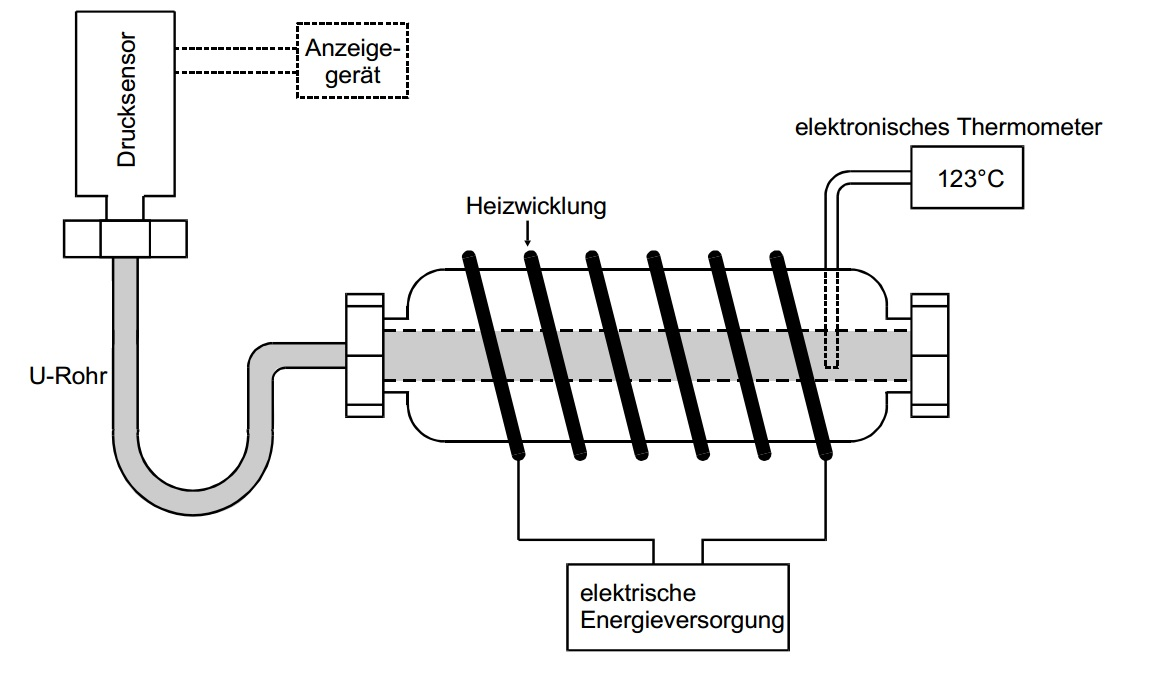
\includegraphics[scale=0.35]{Grafiken/Abb4.jpg}
%        \caption{Schematische Darstellung der Messapparatur aus Versuchsteil 2 Schematische Darstellung der Messapparatur (leicht verändert)}
%        \label{fig:Abb4}
%\end{figure}
